\hypertarget{zeromq}{%
\section{ZeroMQ}\label{zeromq}}

ZeroMQ is an open-source universal messaging library. It will provide a
clean and portable communication API that sits on top of the basic
socket implementation. For us, it means that we can focus our attention
on the communications without getting mired down in the details of the
way the socket is implemented in the language and operating system. It
will help us develop portable code as well as more robust code. ZeroMQ
supports the various communication styles we have discussed (and more).

At this point you may ask, "why not use ROS"? ROS indeed will do what we
need and is vastly popular in the robotics community. This book is about
concepts. With a few exceptions, we are going to develop the programs we
need. We do not need the whole ROS ecosystem. We need interprocess
communications; we need some type of messaging system. ROS is large. ROS
is under active development and can, at times, be challenging to install
as well as use. ZeroMQ is much smaller, with bindings for many languages
and, for us, is a library available to the Python interpreter.

We are only going to touch on ZeroMQ. To really learn about it,
especially for applications outside what we need, please refer to the
Guide: \url{http://zguide.zeromq.org/} . The guide is mostly examples in
C, but enough Python is provided that often you can cut/paste to get
good starting code. Plus, the Python docs address ZeroMQ:
\url{https://pyzmq.readthedocs.io/en/latest/} and
\url{https://learning-0mq-with-pyzmq.readthedocs.io/en/latest/} .

The easiest to understand is the REP pattern. It is a direct peer to
peer client server communication pattern. This is known as REQUEST -
REPLY.

\begin{figure}
\centering
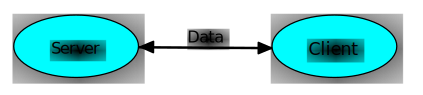
\includegraphics[width=0.5\textwidth,height=\textheight]{ToolsFigures/paircomm.*}
\caption{}
\end{figure}

A basic example is taken from the ZeroMQ guide. Here is a client server
example. The Server code:

\begin{quote}
\# \# Hello World server in Python \# Binds REP socket to tcp://*:5555
\# Expects b"Hello" from client, replies with b"World" \#

import time import zmq

context = zmq.Context() socket = context.socket(zmq.REP)
socket.bind("tcp://*:5555")

\begin{description}
\item[while True:]
\# Wait for next request from client message = socket.recv()
print("Received request: \%s" \% message)

\# Do some 'work' time.sleep(1)

\# Send reply back to client socket.send(b"World")
\end{description}
\end{quote}

And the client:

\begin{quote}
\# \# Hello World client in Python \# Connects REQ socket to
tcp://localhost:5555 \# Sends "Hello" to server, expects "World" back \#

import zmq

context = zmq.Context()

\# Socket to talk to server print("Connecting to hello world
server\ldots") socket = context.socket(zmq.REQ)
socket.connect("tcp://localhost:5555")

\# Do 10 requests, waiting each time for a response for request in
range(10): print("Sending request \%s \ldots" \% request)
socket.send(b"Hello")

\begin{quote}
\# Get the reply. message = socket.recv() print("Received reply \%s {[}
\%s {]}" \% (request, message))
\end{quote}
\end{quote}

Copy these two programs to two files, server.py and client.py. You can
run on the command line using:

\begin{verbatim}
bash> python server.py
\end{verbatim}

and:

\begin{verbatim}
bash> python client.py
\end{verbatim}

Note that control-c will kill the server process. We will go line by
line through the code to understand how this works. To bring in the
ZeroMQ library:

\begin{verbatim}
import zmq
\end{verbatim}

Each process needs a container for the sockets. This container is called
a context:

\begin{verbatim}
context = zmq.Context()
\end{verbatim}

We can create a socket in the context:

\begin{verbatim}
socket = context.socket(zmq.REP)
\end{verbatim}

A socket is a communication conduit. We need to select the communication
protocol (tcp), label the address and select the port (5555):

\begin{verbatim}
socket.bind("tcp://*:5555")
\end{verbatim}

To receive a message:

\begin{verbatim}
message = socket.recv()
\end{verbatim}

To send a message:

\begin{verbatim}
socket.send(b"Hello")
\end{verbatim}

A word about the messages. In Python 3, strings are stored using
Unicode. ZeroMQ uses byte strings, not Unicode. So, we must convert back
and forth from bytes to Unicode. For string literals, place a \emph{b}
in front: b"string". To convert a string variable:

\begin{verbatim}
bmessage = bytes(message,'ascii')
\end{verbatim}

We take the previous example and code up a client server example where
the client sends 10 (x,y) pairs to a server which computes the Two Link
Manipulator Inverse Kinematics for each.

\begin{quote}
import zmq from math import *

context = zmq.Context() socket = context.socket(zmq.REP)
socket.bind("tcp://*:5555")

a1,a2 = 15.0,10.0

\begin{description}
\item[while True:]
\# Wait for next request from client message = socket.recv() list =
message.split(b" ") x = eval(list{[}0{]}) y = eval(list{[}1{]}) d =
(x*x+y*y-a1*a1-a2*a2)/(2*a1*a2) t2 = atan2(-sqrt(1.0-d*d),d) t1 =
atan2(y,x) - atan2(a2*sin(t2),a1+a2*cos(t2)) \# Send reply back to
client reply = bytes(str(t1) + " " + str(t2),'ascii') socket.send(reply)
\end{description}

import zmq import time

context = zmq.Context()

\# Socket to talk to server print("Connecting to IK server\ldots")
socket = context.socket(zmq.REQ) socket.connect("tcp://localhost:5555")

\# Do 10 requests, waiting each time for a response for i in range(10):
x = 5 + 0.2*i y = 3 + 0.3*i print("Compute IK for (\%s,\%s)\ldots" \%
(x,y)) message = bytes(str(x) + " " + str(y),'ascii')
socket.send(message) \# Get the reply. reply = socket.recv()
print("Received reply \%s {[} \%s {]}" \% (i, reply)) time.sleep(0.2)
\end{quote}

And the output is:

\begin{verbatim}
(base) alta:0MQ jmcgough$ python client_IK.py
Connecting to IK server…
Compute IK for (5.0,3.0)…
Received reply 0 [ b'0.9704752657646376 -2.896027136074501' ]
Compute IK for (5.2,3.3)…
Received reply 1 [ b'1.0565361872984023 -2.846929421795498' ]
Compute IK for (5.4,3.6)…
Received reply 2 [ b'1.1267594030030246 -2.802128816232321' ]
Compute IK for (5.6,3.9)…
Received reply 3 [ b'1.185432519250973 -2.7600732877375735' ]
Compute IK for (5.8,4.2)…
Received reply 4 [ b'1.2351575978007627 -2.7199062657491724' ]
Compute IK for (6.0,4.5)…
Received reply 5 [ b'1.277684949617325 -2.681099228530734' ]
Compute IK for (6.2,4.8)…
Received reply 6 [ b'1.3142715256788646 -2.643300360150102' ]
Compute IK for (6.4,5.1)…
Received reply 7 [ b'1.3458611495026371 -2.6062619970976555' ]
Compute IK for (6.6,5.4)…
Received reply 8 [ b'1.373185595974717 -2.569802002720451' ]
Compute IK for (6.8,5.699999999999999)…
Received reply 9 [ b'1.3968260058595374 -2.533781548607152' ]
(base) alta:0MQ jmcgough$
\end{verbatim}

The next model we introduce is the Publisher-Subscriber model which is
nicely supported in 0MQ.

\begin{quote}
Simple PubSub example

import time import zmq

context = zmq.Context() publisher = context.socket(zmq.PUB)
publisher.bind("tcp://*:5555")

i = 0

topic = "Chatter" message = "Hello World" btopic = bytes(topic,'ascii')
bmessage = bytes(message,'ascii')

\begin{description}
\item[while True:]
\begin{description}
\item[\# Do some 'work']
time.sleep(1) i = i+1 print(i)
\item[\# Send reply back to client]
publisher.send\_multipart({[}btopic, bmessage{]})
\end{description}
\end{description}

import zmq

context = zmq.Context()

\# Socket to talk to server print("Connecting to hello world
server\ldots") subscriber = context.socket(zmq.SUB)
subscriber.connect("tcp://localhost:5555")

topic = "Chatter" subscriber.setsockopt\_string(zmq.SUBSCRIBE, topic)

\begin{description}
\item[for r in range(100):]
\# Get the reply. {[}address,message{]} = subscriber.recv\_multipart()
print("Received \%s {[} \%s {]}" \% (r, message))
\end{description}

Simple PubSub example cont.

import time import zmq

context = zmq.Context() publisher = context.socket(zmq.PUB)
publisher.bind("tcp://*:5555")

i = 0

topic1 = "Chatter" message1 = "Hello World" btopic1 =
bytes(topic1,'ascii') bmessage1 = bytes(message1,'ascii')

topic2 = "Chatter2" message2 = "Hello Other World" btopic2 =
bytes(topic2,'ascii') bmessage2 = bytes(message2,'ascii')

\begin{description}
\item[while True:]
\begin{description}
\item[\# Do some 'work']
time.sleep(1) i = i+1 print(i)
\item[\# Send reply back to client]
publisher.send\_multipart({[}btopic1, bmessage1{]})
publisher.send\_multipart({[}btopic2, bmessage2{]})
\end{description}
\end{description}

publisher.close() context.term()

import zmq

context = zmq.Context()

\# Socket to talk to server print("Connecting to hello world
server\ldots") subscriber = context.socket(zmq.SUB)
subscriber.connect("tcp://localhost:5555")

topic = "Chatter"

subscriber.setsockopt\_string(zmq.SUBSCRIBE, topic)

\begin{description}
\item[for r in range(100):]
\# Get the reply. {[}address,message{]} = subscriber.recv\_multipart()
print("Received \%s {[} \%s {]}" \% (r, message))
\end{description}

subscriber.close() context.term()

import zmq

context = zmq.Context()

\# Socket to talk to server print("Connecting to hello world
server\ldots") subscriber = context.socket(zmq.SUB)
subscriber.connect("tcp://localhost:5555")

topic = "Chatter2"

subscriber.setsockopt\_string(zmq.SUBSCRIBE, topic)

\begin{description}
\item[for r in range(100):]
\# Get the reply. {[}address,message{]} = subscriber.recv\_multipart()
print("Received \%s {[} \%s {]}" \% (r, message))
\end{description}

subscriber.close() context.term()
\end{quote}

There are a full range of possibilities here. A program can setup
multiple sockets:

\begin{verbatim}
context = zmq.Context()
publisher = context.socket(zmq.PUB)
publisher.bind("tcp://*:5555")
publisher2 = context.socket(zmq.PUB)
publisher2.bind("tcp://*:5556")
\end{verbatim}

which are published via:

\begin{verbatim}
publisher.send_multipart([btopic1, bmessage1])
publisher2.send_multipart([btopic2, bmessage2])
\end{verbatim}

Likewise one can connect to multiple sockets:

\begin{verbatim}
subscriber = context.socket(zmq.SUB)
subscriber.connect("tcp://localhost:5555")
subscriber2 = context.socket(zmq.SUB)
subscriber2.connect("tcp://localhost:5556")
\end{verbatim}

Which are subscribed via:

\begin{verbatim}
[address,message] = subscriber.recv_multipart()
[address,message] = subscriber2.recv_multipart()







One can easily create multiple data paths.
\end{verbatim}

If you would like the files to act like a program and not require
passing them to Python, then place at the top of the file:

\begin{verbatim}
#!/usr/bin/env python
\end{verbatim}

or:

\begin{verbatim}
#!/usr/bin/env python3
\end{verbatim}

And then make the file executable by:

\begin{verbatim}
chmod +x <filename>
\end{verbatim}
